\chapter{Auswahl elektronischer Komponenten und Verschaltung}\label{ch:komp}
Im Folgenden wird auf die Auswahl der Platinenkomponenten, sowie deren Beschaltung eingegangen. Der gesamte Schaltplan ist in \autoref{app:boardlayout} angefügt.
\section{Anforderungen an die Komponenten}
Elektronische Komponenten sind üblicherweise in passive und aktive Bauelemente untergliedert. Unter passiven Bauelementen werden Komponenten verstanden, die das Eingangssignal ohne Verstärkung übertragen. Aktive Bauelemente benötigen meist eine Hilfsquelle und können somit ein Eingangssignal verstärken \cite[S.25]{haendschke}. Für den Einsatz elektronischer Komponenten im Automobilbereich hat sich für passive Bauteile die Zertifizierung nach AEC-Q200 und für aktive Bauteile die nach AEC-Q100 als Qualitätsstandard etabliert. Anhand dieser Zertifizierungen wird eine nachweisliche Belastbarkeit der Bauelemente nach dem jeweiligen Standard definiert. Für die Anforderungen an die Platine werden die passiven Bauelemente nach AEC-Q200 und die aktiven Bauelemente nach AEC-Q100 mindestens in \textit{Grade 2} eingestuft, um den Temperaturanforderung bis \SI{105}{^\circ C} gerecht zu werden \cite[S.6]{aecq}. 
\subsection{Passive Bauteile}
Unter die benötigten passiven Bauteile fallen Kondensatoren und Widerstände, welche nach dem AEC-Q200 Standard ausgewählt werden. Anforderung ist danach eine thermische Belastbarkeit von mindestens \SI{105}{^\circ C}. Um eine geringe Baugröße der Platine zu gewährleisten, sollten sowohl Widerstände als auch Kondensatoren als SMD-Bauteil (\textit{surface-mounted device}) gewählt werden. Für Abblockkondensatoren werden nach \cite[S.7]{ldo} Keramikkondensatoren mit XR7 präferiert. Diese werden einerseits dazu genutzt, um bei impulsartiger Netzbelastung durch hohe Leistungsaufnahme von ICs das Netz zu entlasten, andererseits aber auch um Restwelligkeiten zu filtern. Als Baugröße bei manueller Bestückung bieten sich die Standardgrößen 1206 oder 0805 (Angabe in $\frac{1}{100}$ Zoll) an, welche noch per Hand lötbar sind. Die Widerstände für die Sensorik müssen mit sehr hoher Präzision, geringem Rauschen und niedriger Temperaturabhängigkeit gewählt werden, um Messfehler aufgrund falscher Widerstandswerte zu vermeiden. Im Anwendungsfall bieten sich daher Dünnschichtwiderstände an.
\subsection{Aktive Bauteile}
Die aktiven Bauelemente der Platine müssen dafür ausgelegt werden, im Späteren alle Anforderungen aus der Anforderungsliste (vgl. \autoref{tab:Anforderungsliste}) gerecht zu werden. Demnach müssen sie in ihrer logischen Verschaltung einerseits in der Lage sein den Tauchspulenaktor anzusteuern und auszuregeln, andererseits aber auch die Bedingungen über Leistungsaufnahme etc. erfüllen. Kern der Platine ist ein Mikrocontroller, welcher schnell genug sein muss, um Gangwechsel in weniger als \SI{0,1}{s} durchzuführen. Weiterhin muss der Mikrocontroller die CAN-Kommunikation mit der MicroAutobox unterstützen. Da der Mikrocontroller nicht über die \SI{13,8}{V} der Autobatterie gespeist werden kann, wird ein Spannungsregler benötigt, welcher auf die Betriebsspannung des Mikrocontrollers regelt. Um aus den physikalischen Bussignalen CAN-HIGH und CAN-LOW für den Mikrocontroller verwertbare Signale zu erhalten wird ein CAN-Transciever benötigt. Über diesen ist eine Kommunikation des Mikrocontrollers mit der CAN-Peripherie erst möglich. Zum Regeln des Tauchspulenaktors ist ein Motortreiber nötig, welcher vom Mikrocontroller angesteuert wird, um die Spannung an den Tauchspulenaktor durchzuschalten. Eine Ansteuerung des Motortreibers mittels PWM-Signal sollte möglich sein. Der Motortreiber muss dabei für zukünftige Aktorkonfigurationen für Ströme bis zu \SI{55}{A} ausgelegt sein. Des Weiteren wird eine Spannungsebene von \SI{5}{V} benötigt um die Lagesensorik des Aktors zu unterstützen, wofür ein zweiter Spannungsregler eingeplant werden muss.
%\begin{figure}[H]%
%\centering
%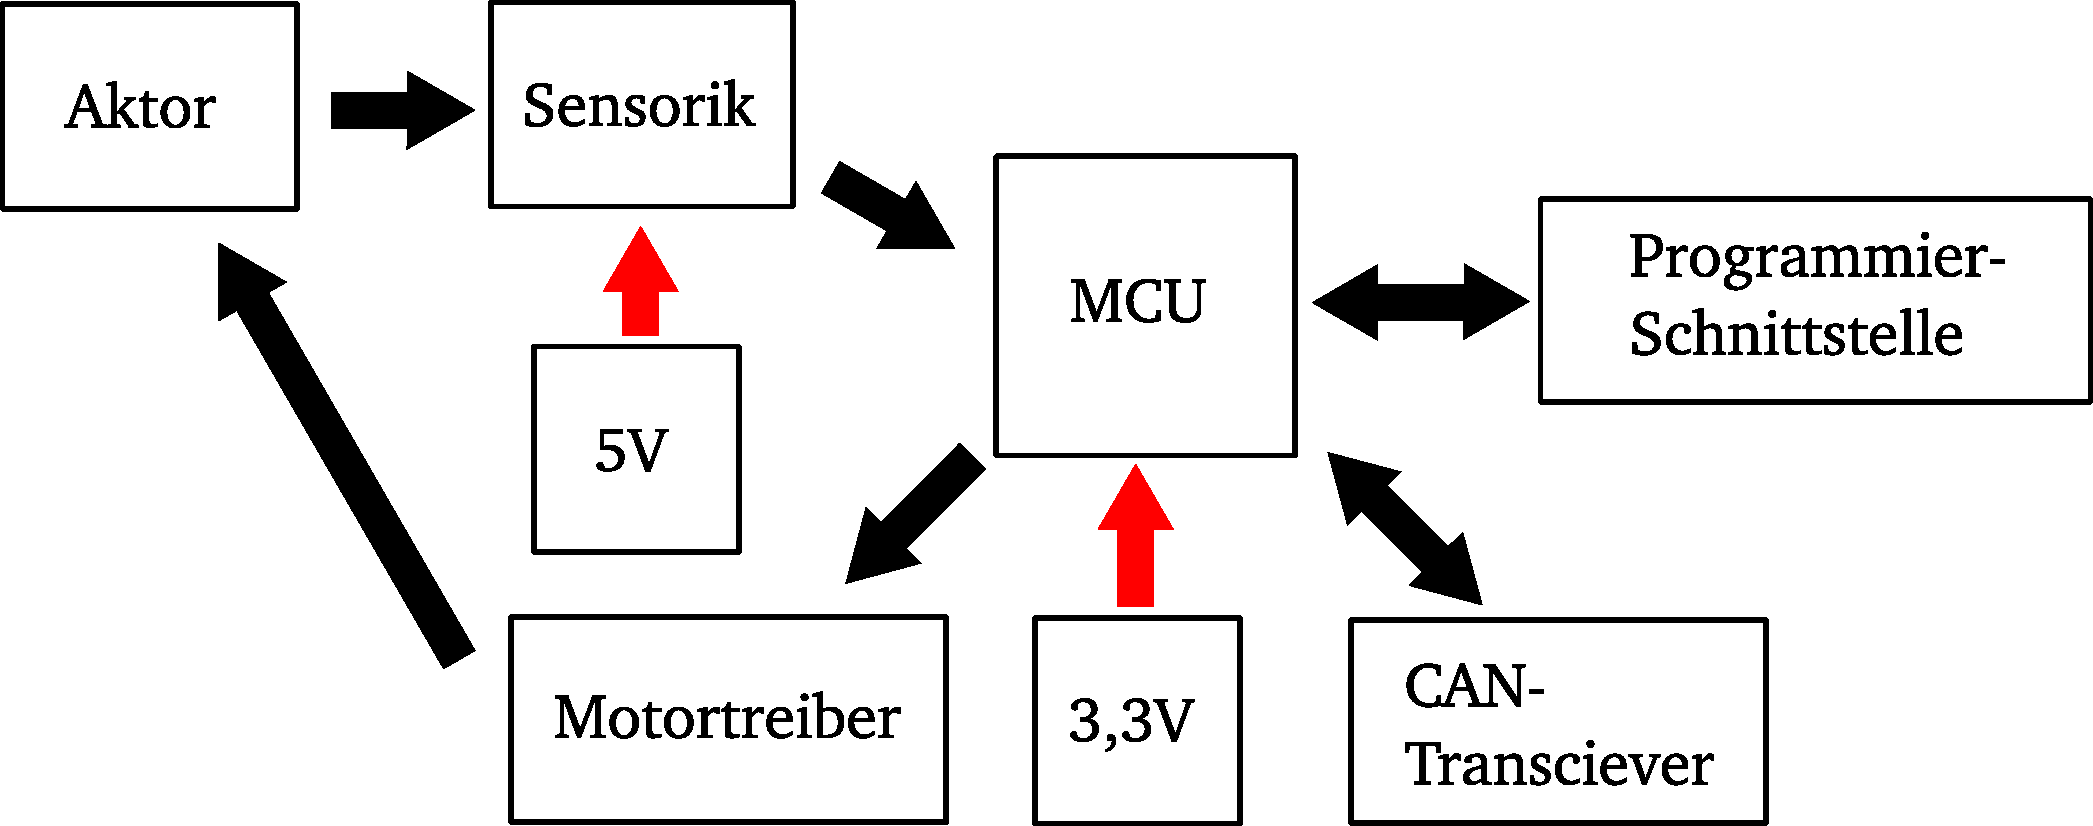
\includegraphics[width=250pt]{./Bilder/anf.pdf}%
%\caption{Benötigte Ebenen der Verschaltung}%
%\label{fig:anf}%
%\end{figure}
\newpage
\section{Komponentenauswahl}
Anhand der Anforderungen an die Platinenelemente sind die endgültigen Komponenten der Platine zu wählen. Es müssen Mikrocontroller, Spannungsregler, CAN-Transciever und Motortreiber ausgewählt werden. Weiterhin wird eine Temperaturbeständigkeit bis \SI{105}{^\circ C} gefordert.
\subsection{Mikrocontroller}\label{sec:mcu_kap4}
Die Recheneinheit zur Regelung des Tauchspulenaktors ist ein STM32F405RGT7-Mikrocontroller. Dieser ist mit verschiedenen Pin-Anzahlen erhältlich und auf der Platine aus Platzgründen in der Ausführung LQFP64 mit 64 Pins verbaut. Der Mikrocontroller zeichnet sich durch seine hohe CPU-Geschwindigkeit von \SI{168}{MHz} und seine große Programm-Speichergröße von \SI{1}{MB} aus. Die Namensendung -T7 steht dabei für die zulässige Betriebstemperatur von -40...\SI{105}{^\circ C}. Weiterhin besitzt dieser Mikrocontroller die geforderten CAN-Schnittstellen, anhand derer mit der MicroAutobox kommuniziert werden soll. In \autoref{fig:mcumin} ist die Minimalbeschaltung des Mikrocontrollers zu sehen. Diese ist dem Datenblatt des STM32 entnommen \cite[S.77]{stm32} (vgl. \autoref{app:stm32man}). Die Pins mit den Bezeichnungen VDD bis VDD\_4 sind die Versorgungspins des Mikrocontrollers. An diesen Pins liegt die Versorgungsspannung an, welche nach dem Datenblatt zwischen 1,8 und \SI{3,6}{V} liegt. Diese ist aufgrund der Versorgungsspannung anderer Bauteile zu VDD = \SI{3,3}{V} gewählt. Die VDD Pins werden durch die Keramikkondensatoren C7 bis C11 entkoppelt, welche nach dem Datenblatt dimensioniert sind und möglichst nah an den dem jeweiligen VDD-Pin plaziert werden sollen. Die Entkopplung wird benötigt, um Welligkeiten der Spannungsversorgung zu filtern und parasitäre Induktivitäten zu entkoppeln \cite{decoupling}. Der Pin VBAT wird unter anderem für die Versorgung der Echtzeituhr (\textit{RTC}), der Backup-Register und des Backup-SRAMs genutzt und wird, wenn keine zweite Spannungsversorgung neben der Hauptversorgung vorhanden ist, ebenfalls an VDD angeschlossen \cite[S.31]{stm32}. VDDA ist der Pin für die Spannungsversorgung des Analog-Digital-Converters (\textit{ADC}) und wird ebenfalls mit der Versorgungsspannung von VDD angeschlossen. Die Kapazitäten C5 und C6 sind nach den Herstellerangaben dimensioniert und sorgen ebenfalls für eine Entkopplung der Spannungsversorgung. Die Induktivität L1 bietet die Möglichkeit, je nach Welligkeit der Versorgungsspannung, diese über einen LC-Filter zu filtern um eine bessere Auflösung des ADCs zu gewährleisten. Wenn dieser Filter nicht benötigt wird, sollte L1 durch einen \SI{0}{\Omega} Widerstand ersetzt werden.
VCAP\_1 und VCAP\_2 sind die Ausgänge des internen Voltage Regulators des STM32 und C5 bzw. C6 werden zur Glättung der intern geregelten Spannung genutzt \cite[S.77]{stm32}. Die Pins VSS, VSS\_2 und VSSA sind die GND Anschlüsse für den Mikrocontroller und den internen ADC.
\begin{figure}[H]%
\centering
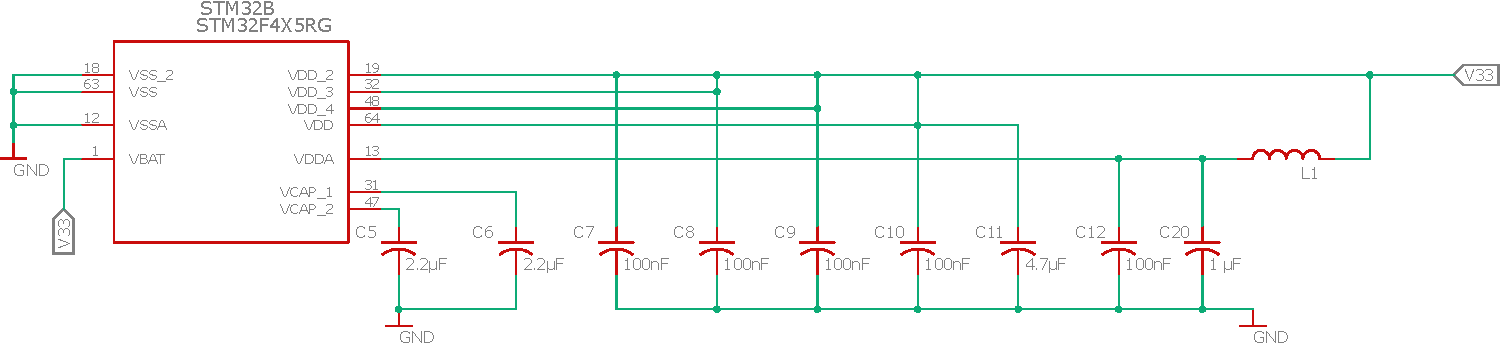
\includegraphics[width=\columnwidth]{./Bilder/MCU_MIN.pdf}%
\caption{Minimalbeschaltung des STM32F405RGT7}%
\label{fig:mcumin}%
\end{figure}\noindent
In \autoref{fig:mcupin} sind die Pin-Belegungen des Mikrocontrollers dargestellt, welche durch \autoref{tab:pins} genauer beschrieben sind. Unter Sensorik fallen die Ausgänge für Lagesensorik, Temperatursensorik und Messung der Versorgungsspannung. Die UART Pins können zum \textit{debuggen} auf der endgültigen Platine genutzt werden. Zur CAN-Kommunikation werden die Pins CAN1-TX (PA11) und CAN1-RX (PA12) benötigt, womit der Mikrocontroller über einen CAN-Transciever Nachrichten an die MicroAutobox senden und ebenfalls Nachrichten von dieser empfangen kann. Zum Programmieren des Mikrocontrollers wird eine \textit{SWD}-Schnittstelle aufgebaut, welche sich mittels externem ST-Link/V2 mit dem Computer verbinden lässt. Dazu werden die jeweiligen Pins über den Platinenstecker nach außen geführt (vgl. \autoref{fig:stecker}). Weiterhin müssen Pins zum Beschalten der H-Brücke und zum Auslesen der Strommessungen belegt werden. Die Pins OSC\_IN und OSC\_OUT sind zum Anschließen eines externen Quarzes, welcher als Taktgeber für den Mikrocontroller genutzt wird. Der Pin NRST wird für den Fall eines notwendigen Resets herausgeführt. Über diesen kann der Mikrocontroller bei Fehlern im Befehlszähler (\textit{program counter corruption}) wieder in den Initialzustand des Programms zurückgesetzt werden. Daten aus dem Flash-Speicher bleiben dabei unverändert. Dazu muss der NRST-Pin für eine Sekunde extern auf \textit{low} (0 bis \SI{0,8}{V}) gezwungen werden \cite[S. 111]{stm32}. Somit ist im Falle eines undefinierten Programmzustands auch im eingebauten System ein Programmneustart ohne Datenverlust möglich.

\noindent\begin{minipage}{0.75\textwidth}
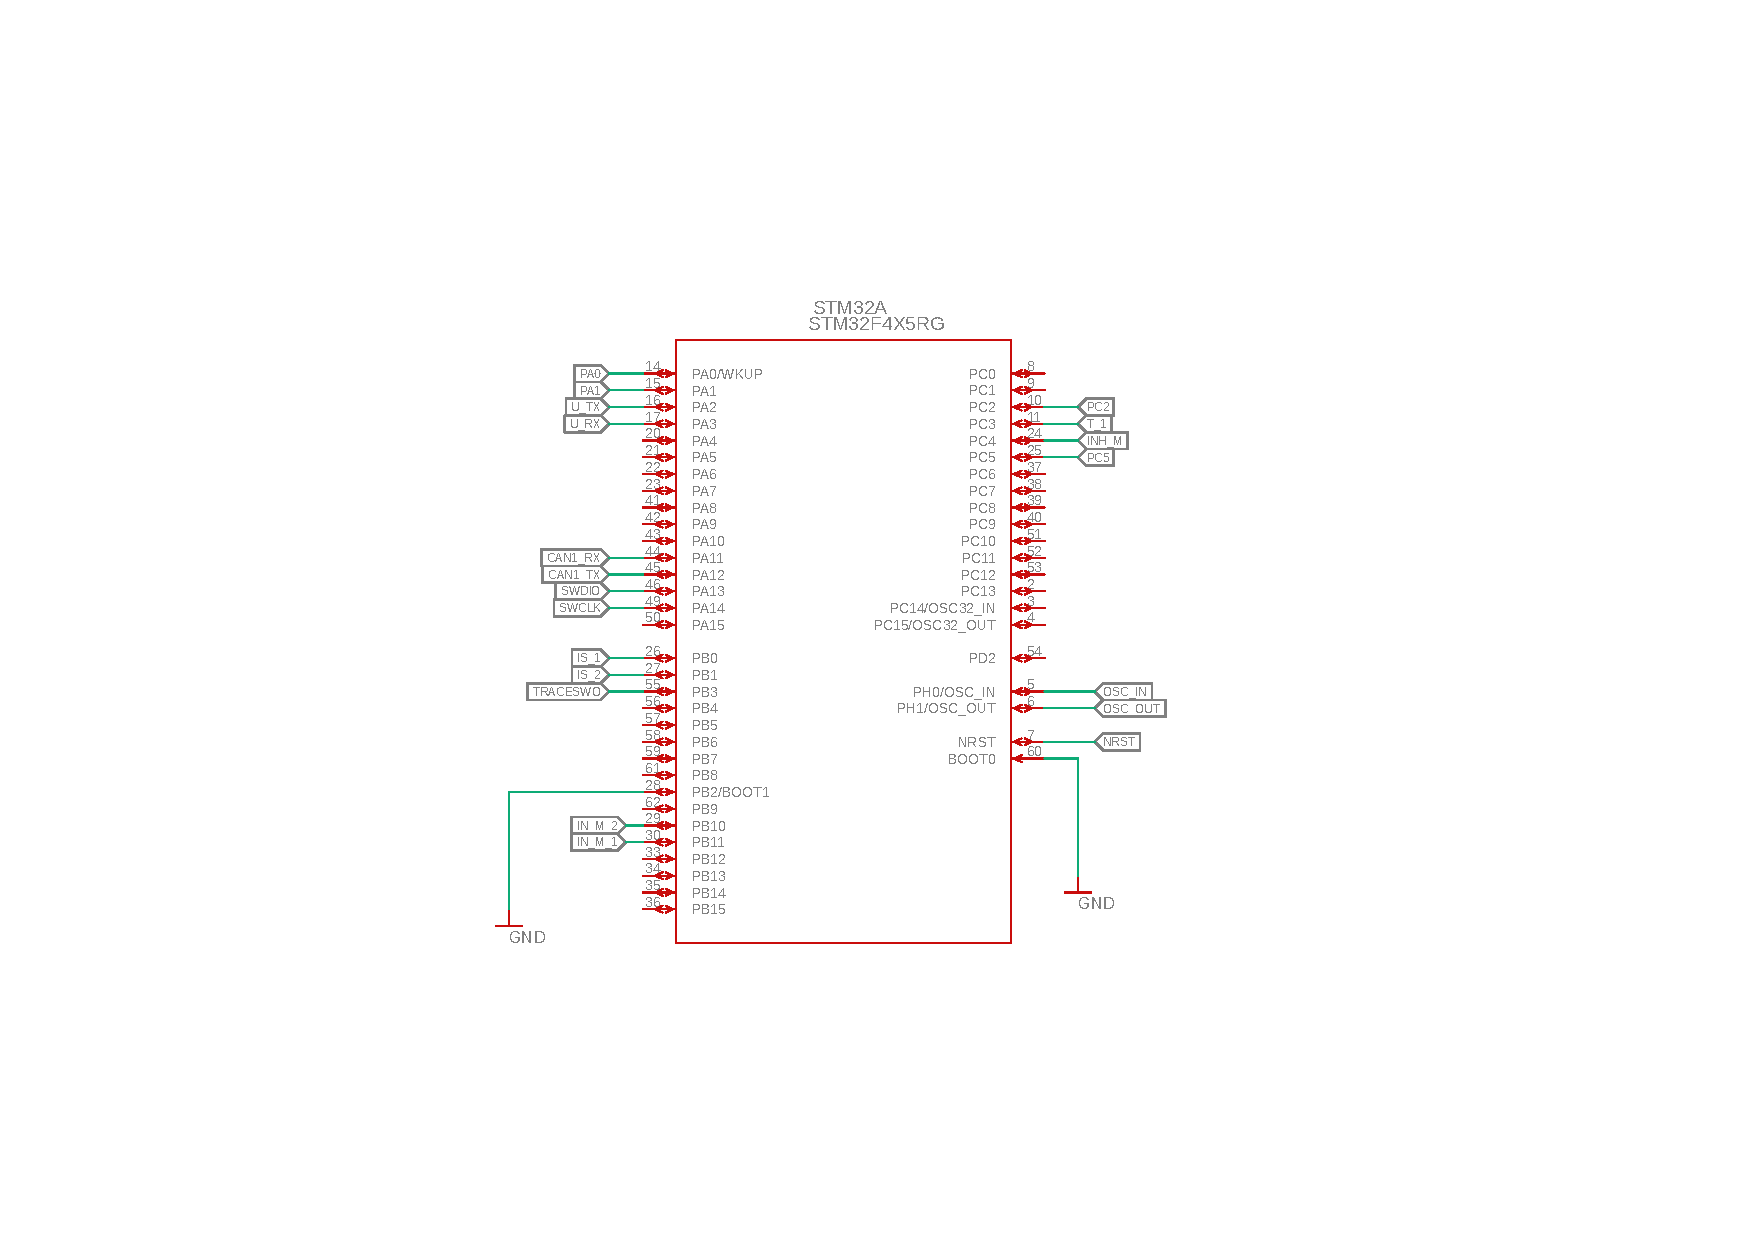
\includegraphics[width=\textwidth]{./Bilder/MCU_PINS.pdf}
\end{minipage}
\noindent\begin{minipage}{0.1\textwidth}
\begin{tabular}{l | l}
			Pin & Funktion\\ \hline
			PA0& Sensorik\\
			PA1& Sensorik\\
			PB0& Sensorik\\
			PB1& Sensorik\\
			PC2& Sensorik\\
			PC3& Sensorik\\
			PC5& Sensorik\\
			PA2& UART\\
			PA3& UART\\
			PA11& CAN\\
			PA12& CAN\\
			PA13&SWD\\
			PA14&SWD\\
			PB3& SWD\\
			PB0 & H-Brücke\\
			PB1 &H-Brücke\\
			PB10&H-Brücke\\
			PB11&H-Brücke\\
			PC4&H-Brücke\\
			OSC\_IN&Quarz\\
			OSC\_OUT&Quarz\\
			NRST & Reset
		\end{tabular}
\end{minipage}

\noindent\begin{minipage}{0.75\textwidth}
\captionof{figure}{Pin-Belegung des Mikrocontrollers}
\label{fig:mcupin}
\end{minipage}
\noindent\begin{minipage}{0.2\textwidth}
	\captionof{table}{Pin-outs}
	\label{tab:pins}
\end{minipage}
\hspace{1cm}
\newline
\\
Wichtig bei der Beschaltung ist außerdem die Belegung von BOOT0 und BOOT1, welche den Speicherbereich definieren, aus dem der Mikrocontroller beim Startvorgang sein Programm lädt. Nach \autoref{tab:boot} muss für den Start im Main Flash memory BOOT0 auf GND-Niveau gesetzt werden, während die Belegung von BOOT1 undefiniert ist und somit mit GND belegt werden kann.

\begin{table}[H]%
\centering
\captionabove{Boot modes des STM32F405RGT7 nach \cite[S.69]{stmref}}
\begin{tabular}{c c c c}
BOOT1 & BOOT0 & Boot mode & Aliasing \\ \hline
x & 0 & Main Flash memory & Main Flash memory is selected as the boot space\\
0 & 1 & System memory & System memory is selected as the boot space\\
1 & 1 & Embedded SRAM & Embedded SRAM is selected as the boot space
\end{tabular}

\label{tab:boot}
\end{table}\noindent
Um möglichst akurate Taktraten zu haben und somit Schaltvorgänge und Sensorikdaten genau und reproduzierbar zu gestalten, wird, wie vom Hersteller des Mikrocontrollers empfohlen, ein externer Taktgeber benutzt \cite[S.218]{stmref}. Auf der Platine wird hierbei ein ABLS-8.000MHZ-K4T von Abracon genutzt, welcher eine Nennfrequenz von 8MHz hat. \autoref{fig:quarz} zeigt die letztendliche Verschaltung auf der Platine. Die Lastkapazitäten CQ1 und CQ2 von \SI{22}{pF} sind dabei nach dem Datenblatt des Herstellers gewählt. Die Widerstände R19 und R20 sind einerseits verbaut, um den externen Quarz vom Mikrocontroller trennen zu können, andererseits wird R20 benutzt, um den Stromfluss des Quarzes zu beschränken \cite[S.16]{stmquarz}. Nach \cite[S.16]{stmquarz} lässt sich eine Abschätzung von R20 über
\begin{align*}
R_{20} = \frac{1}{2\pi f C_{Q1}}
\end{align*}
gewinnen. Damit ergibt für R20 sich ein Richtwert von etwa \SI{900}{\Omega} bei CQ1 = 22pF. Ein zu niedriger Widerstand erhöht die Verlustleistung über den Quarz, während ein höherer Widerstand zum Stillstand der Oszillation führen kann. Auf der Platine ist ein Widerstand von \SI{1}{k\Omega} gewählt.

\begin{figure}[H]%
\centering
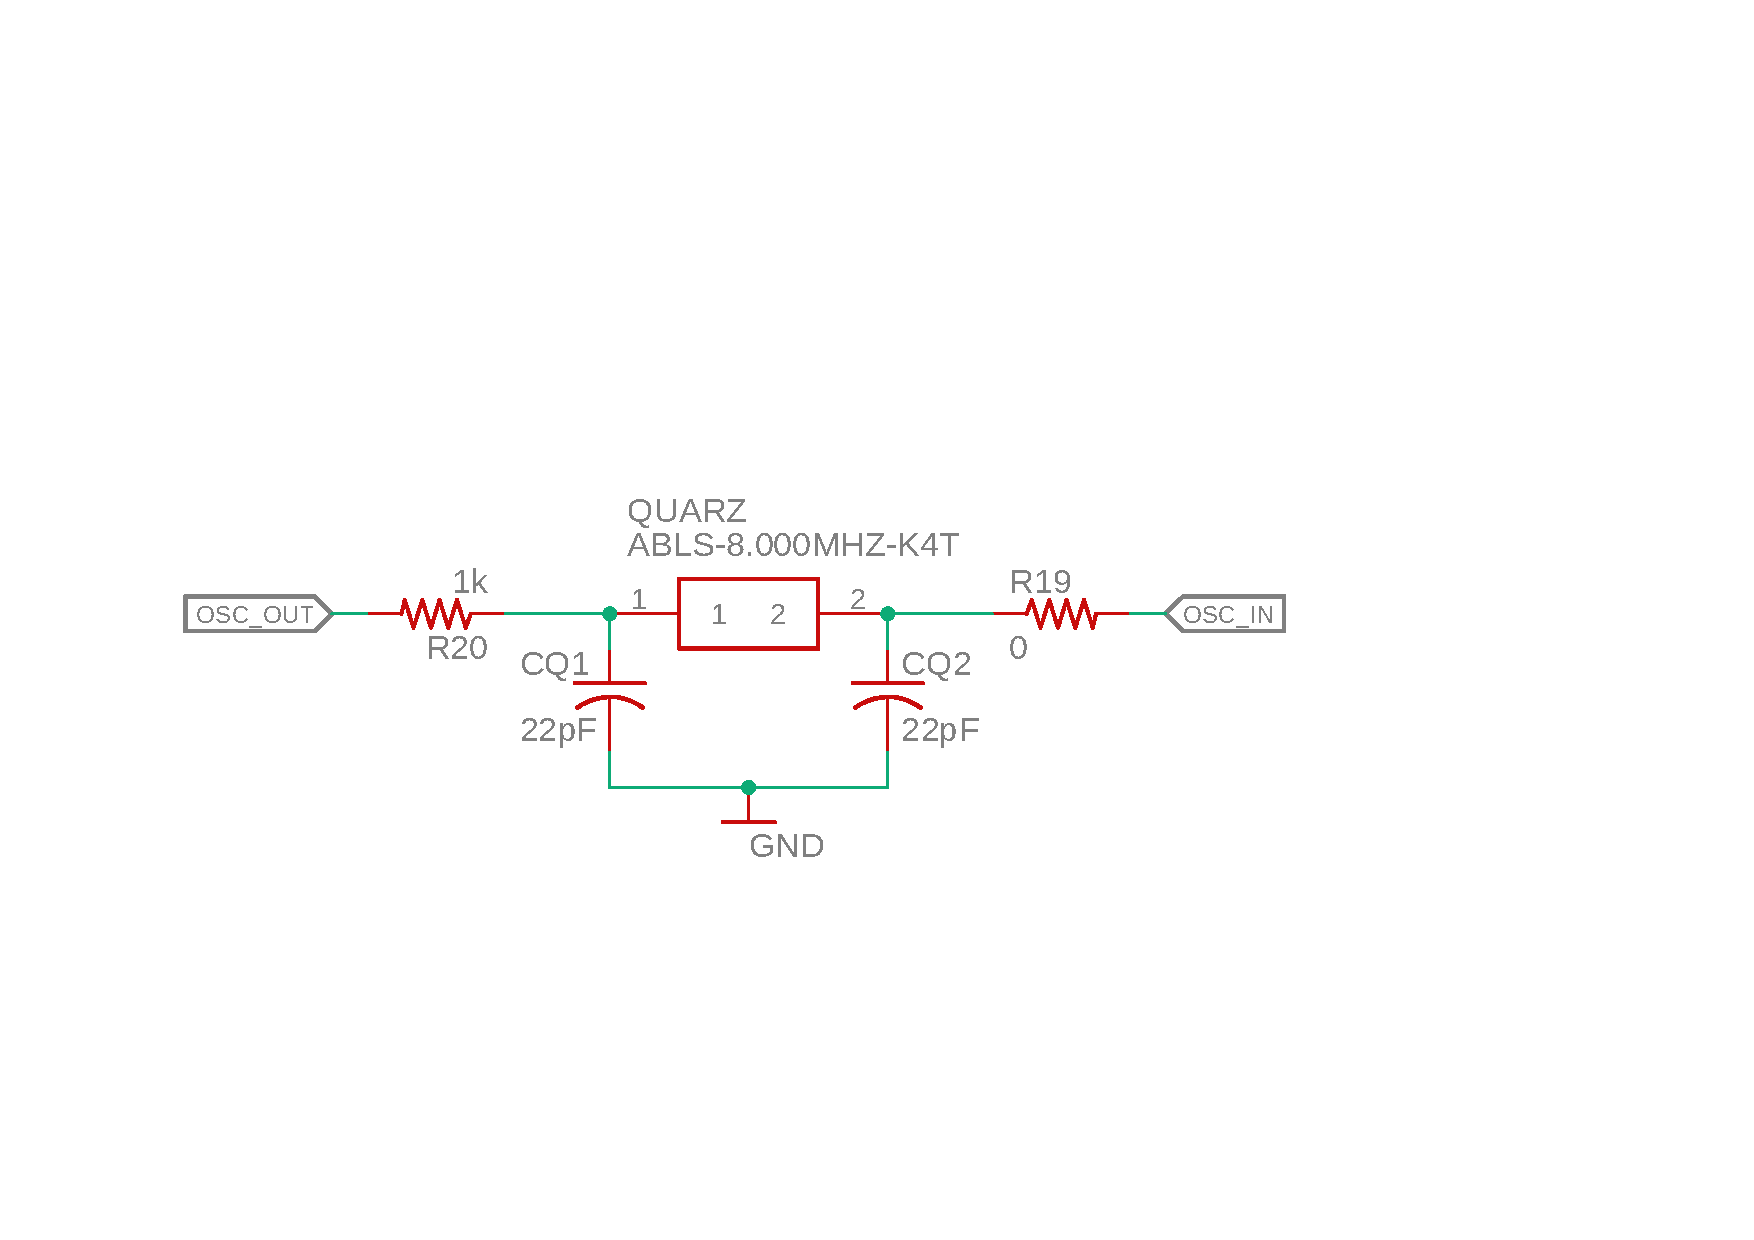
\includegraphics[width=300pt]{./Bilder/quarz.pdf}%
\caption{Anschluss externer Quarz}%
\label{fig:quarz}%
\end{figure}

\subsection{CAN-Transciever}
Zur Kommunikation des Mikrocontrollers mit der MicroAutobox ist eine Signalübertragung über CAN vorgesehen. Da der Mikrocontroller die physikalischen Bussignale nicht verarbeiten kann, wird die Kommunikation des Mikrocontrollers mit dem Bussystem über einen CAN-Transciever gestaltet. Dieser sorgt dafür, dass den Mikrocontroller nur für ihn lesbare Daten erreichen und übersetzt gleichzeitig die vom Mikrocontroller ins Bussystem gesendeten Nachrichten. Die Pins des Mikrocontrollers für diese Aufgaben sind CAN1-RX zum Erhalten von Informationen und CAN1-TX zum Senden von CAN-Nachrichten. Auf Busebene gibt es die Signale CAN-HIGH und CAN-LOW, welche in \autoref{sec:CAN_KAP2} beschrieben wurden. In \autoref{fig:cantrans} ist die Verschaltung des CAN-Transcievers SNHVD230QD von Texas Instruments zu sehen. An Pin VCC wird die Spannungsversorgung von \SI{3,3}{V} angeschlossen. VREF ist ein Ausgangspin mit halber VCC-Spannung beispielsweise zum Entwerfen einer Split-Termination. Pin D ist der Anschlusspin für die gesendeten Nachrichten des Mikrocontrollers über CAN1-TX. Pin R sendet die übersetzten CAN-Nachrichten des Bussystems an CAN1-RX.
\begin{figure}[H]%
\centering
\includegraphics[width=400pt]{./Bilder/can.pdf}%
\caption{CAN-Transciever Verschaltung}%
\label{fig:cantrans}%
\end{figure}\noindent
Über den Pin RS lassen sich durch den Widerstand R\_RS verschiedene \textit{slew rates} einstellen und damit, wie schnell der Ausgangstransistor bei der Übermittlung von Nachrichten durchschaltet \cite[S. 2]{cantrans}. Für einen Widerstandswert von \SI{0}{\Omega} ist die Geschwindigkeit maximal, während sie bei \SI{10}{k\Omega} etwa \SI{15}{\frac{V}{\mu s}} beträgt. Zwischen CAN-HIGH und CAN-LOW wird nach dem Datenblatt ein \SI{120}{\Omega} geschaltet. Bei der Wahl von R5 und R\_RS wurde sich an der bestehenden Konfiguration des STM-Discovery-Shields orientiert, mit der die CAN-Kommunikation aufgebaut wurde. 

\subsection{Spannungsversorgung}\label{sec:spannver}
Die Elektronik wird weiterhin mit dem bisher verwendeten Manson SBC-2130 Battery Charger versorgt. Dieser stellt eine konstante Spannung von \SI{13,8}{V}. Da die verschiedenen Komponenten jedoch Versorgungsspannungen von \SI{3,3}{V} und \SI{5}{V} benötigen, muss die Schaltung durch einen Spannungsregler erweitert werden. Zusätzlich werden dadurch Schwankungen in der Eingangsspannung geglättet. 
\subsubsection{Low Dropout Spannungsregler}
Ein Low Dropout Spannungsregler (\textit{LDO}) ist ein Festspannungsregler, der eine festgelegte und somit invariable Ausgangsspannung liefert, die sich auch dann nicht ändert, wenn die Eingangsspannung schwankt. Die Schaltung eines LDO-Reglers besteht aus einer Referenzspannungsquelle, einem Differenzverstärker und einem Stellglied in Form eines Leistungstransistors. Die hier verwendeten Ausführungen sind P-Kanal-MOSFET-basierte Regler. Das Blockschaltbild eines solchen LDOs ist in folgender Abbildung schematisch dargestellt.\\
\begin{figure}[H]
	\centering
		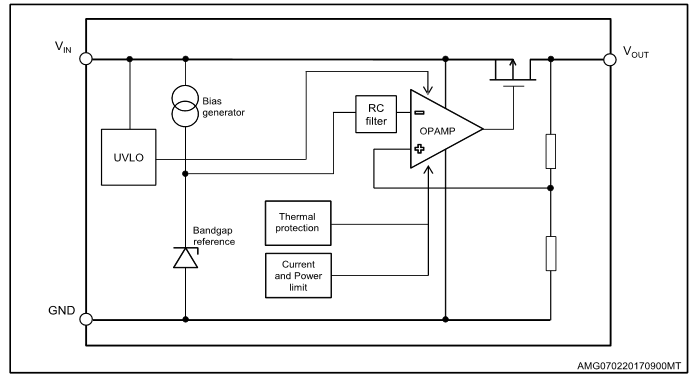
\includegraphics[width=350pt]{./Bilder/LDO.png}
	\caption{Blockschaltbild LDO nach \cite{ldo}}
	\label{fig:LDO2}
\end{figure} \noindent
Der Differenzverstärker vergleicht die Ausgangsspannung mit einer stabilen Referenzquelle aus einer Zenerdiode, sodass die gemessene Spannungsabweichung über das Stellglied ausgeregelt werden kann. Ist die Ausgangsspannung zu niedrig, so wird der Transistor stärker angesteuert bis die geforderte Ausgangsspannung erreicht wird. Im umgekehrten Fall wird der Strom über den Transistor reduziert. Der Transistor wird in dieser Schaltung wie ein veränderlicher Widerstand verwendet, an dem die überflüssige Spannungsdifferenz abfällt und in Wärme umgewandelt wird. Die verwendeten LDOs besitzen außerdem eine Strombegrenzungsschaltung, eine Unterspannungsabschaltung sowie eine Schutzschaltung, die die Betriebstemperatur überwacht und das Bauteil vor thermischer Überlastung schützt. 
\subsubsection{Verschaltung auf Platine}
Grund für die Wahl dieser Art von Spannungsreglern für die Platine ist ihre kompakte Bauform, ihr günstiger Einkaufspreis und das geringe Rauschen im Vergleich zu Schaltreglern, da keine Schaltvorgänge auftreten. Auf der Platine werden LDOs vom Typ LDL1117 von STMicroelectronics verwendet. Für die \SI{3,3}{V} Versorgung ist dies der LDL1117S33R und für die \SI{5}{V} der LDL1117S50R LDO. Nach dem Datenblatt \cite[S.7]{ldo} ist die Eingangskapazität zu \SI{1}{\mu F} und die Ausgangskapazität zu \SI{4,7}{\mu F} zu wählen. Diese werden aus Stabilitätsgründen und zur Entkopplung verwendet. Empfohlen wird weiterhin Keramikkondensatoren zu verwenden, welche X5R oder X7R Dielektrika aufweisen. In \autoref{fig:volt} ist der Schaltplan der Spannungsversorgung für die Platine zu sehen. An VIN wird die Batteriespannung angelegt, welche mit \SI{1}{\mu F} gegen GND entkoppelt wird. An VOUT liegen die jeweiligen \SI{3,3}{V} bzw. \SI{5}{V} an, welche jeweils über \SI{4,7}{\mu F} gegen GND geschaltet sind. Zur allgemeinen Spannungsglättung wird eine Kapazität C13 von \SI{1000}{\mu F} zwischen der Batteriespannung und GND geschaltet, welche starke Schwankungen beim Durchschalten der H-Brücke verhindern soll.

\begin{figure}[H]%
\centering
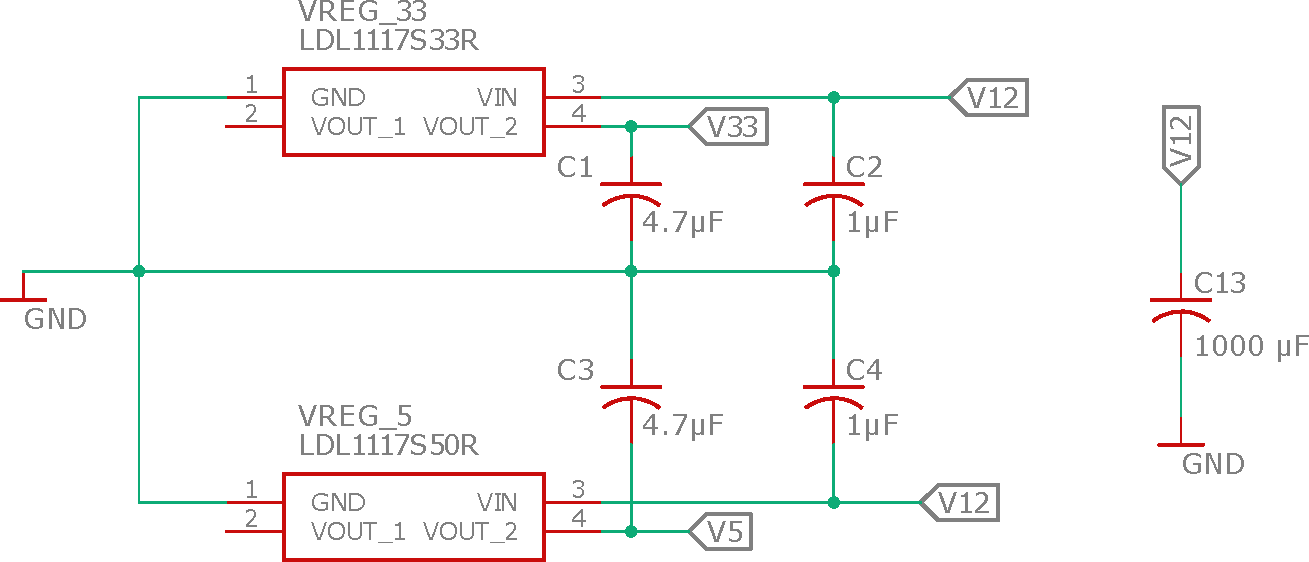
\includegraphics[width=410pt]{./Bilder/volt.pdf}%
\caption{Schaltplan Spannungsversorgung}%
\label{fig:volt}%
\end{figure}

\section{Platinenanschluss}\label{sec:stecker}
Die Platine wird mit einem 1-776267-1 Stecker von TE Connectivity verbunden, um notwendige Signalleitungen nach Außen zu führen und zusätzlich Spannungsversorgung und Lagesensorik mit der Platine verbinden zu können. In \autoref{fig:stecker} ist die Pin-Belegung des Steckers zu sehen. Um den Mikrocontroller über SWD programmieren zu können, muss der Stecker die notwendigen Signalleitungen SWDIO, SWCLK, TRACESWO, V33 und GND nach Außen führen. Diese werden direkt mit einem ST-Link/V2 nach \autoref{app:stlink} verbunden, sodass Programme von einem Computer auf den Mikrocontroller übertragen werden können. Zusätzlich muss der Mikrocontroller zur Programmierung mit Spannung versorgt werden, sodass der Stecker mit der Autobatterie verbunden sein muss. Weiterhin soll der Mikrocontroller über CAN-Signale mit der MicroAutobox kommunizieren können. Dazu werden die Schnittstellen CANH (CAN-HIGH) und CANL (CAN-LOW) über den Stecker nach außen geführt. Die Steckerpins V5, L\_1, L\_2 und GND werden für die Lagesensorik benötigt. Pin 4 und Pin 5 sind beide mit der Batterie verbunden und bilden die Spannungsversorgung der gesamten Platine. Aufgrund der potentiell hohen Ströme wird die Versorgung über zwei Pins zugeführt. Über den NRST-Pin lässt sich der Mikrocontroller zurücksetzen (vgl. \autoref{sec:mcu_kap4}).\\ Als Gegenstück des Steckers existieren drei verschiedene Varianten. Jeweils eine Variante sind Programmier- und Betriebsstecker, die dritte Variante vereint diese beiden Optionen. Der Programmierstecker beinhaltet dabei alle Eingänge der oben genannten Signalleitungen, die zum Flashen des Mikrocontrollers über SWD nötig sind, und wird nur kurzzeitig verwendet. Im Dauerbetrieb wird der Betriebsstecker verbunden, welcher die Leitungen zur Spannungsversorgung, Lagesensorik und CAN-Kommunikation führt. Der kombinierte Stecker ist vor allem in der Entwicklungsphase hilfreich, um nicht ständig den Anschluss wechseln zu müssen. 


\begin{figure}[H]%
\centering
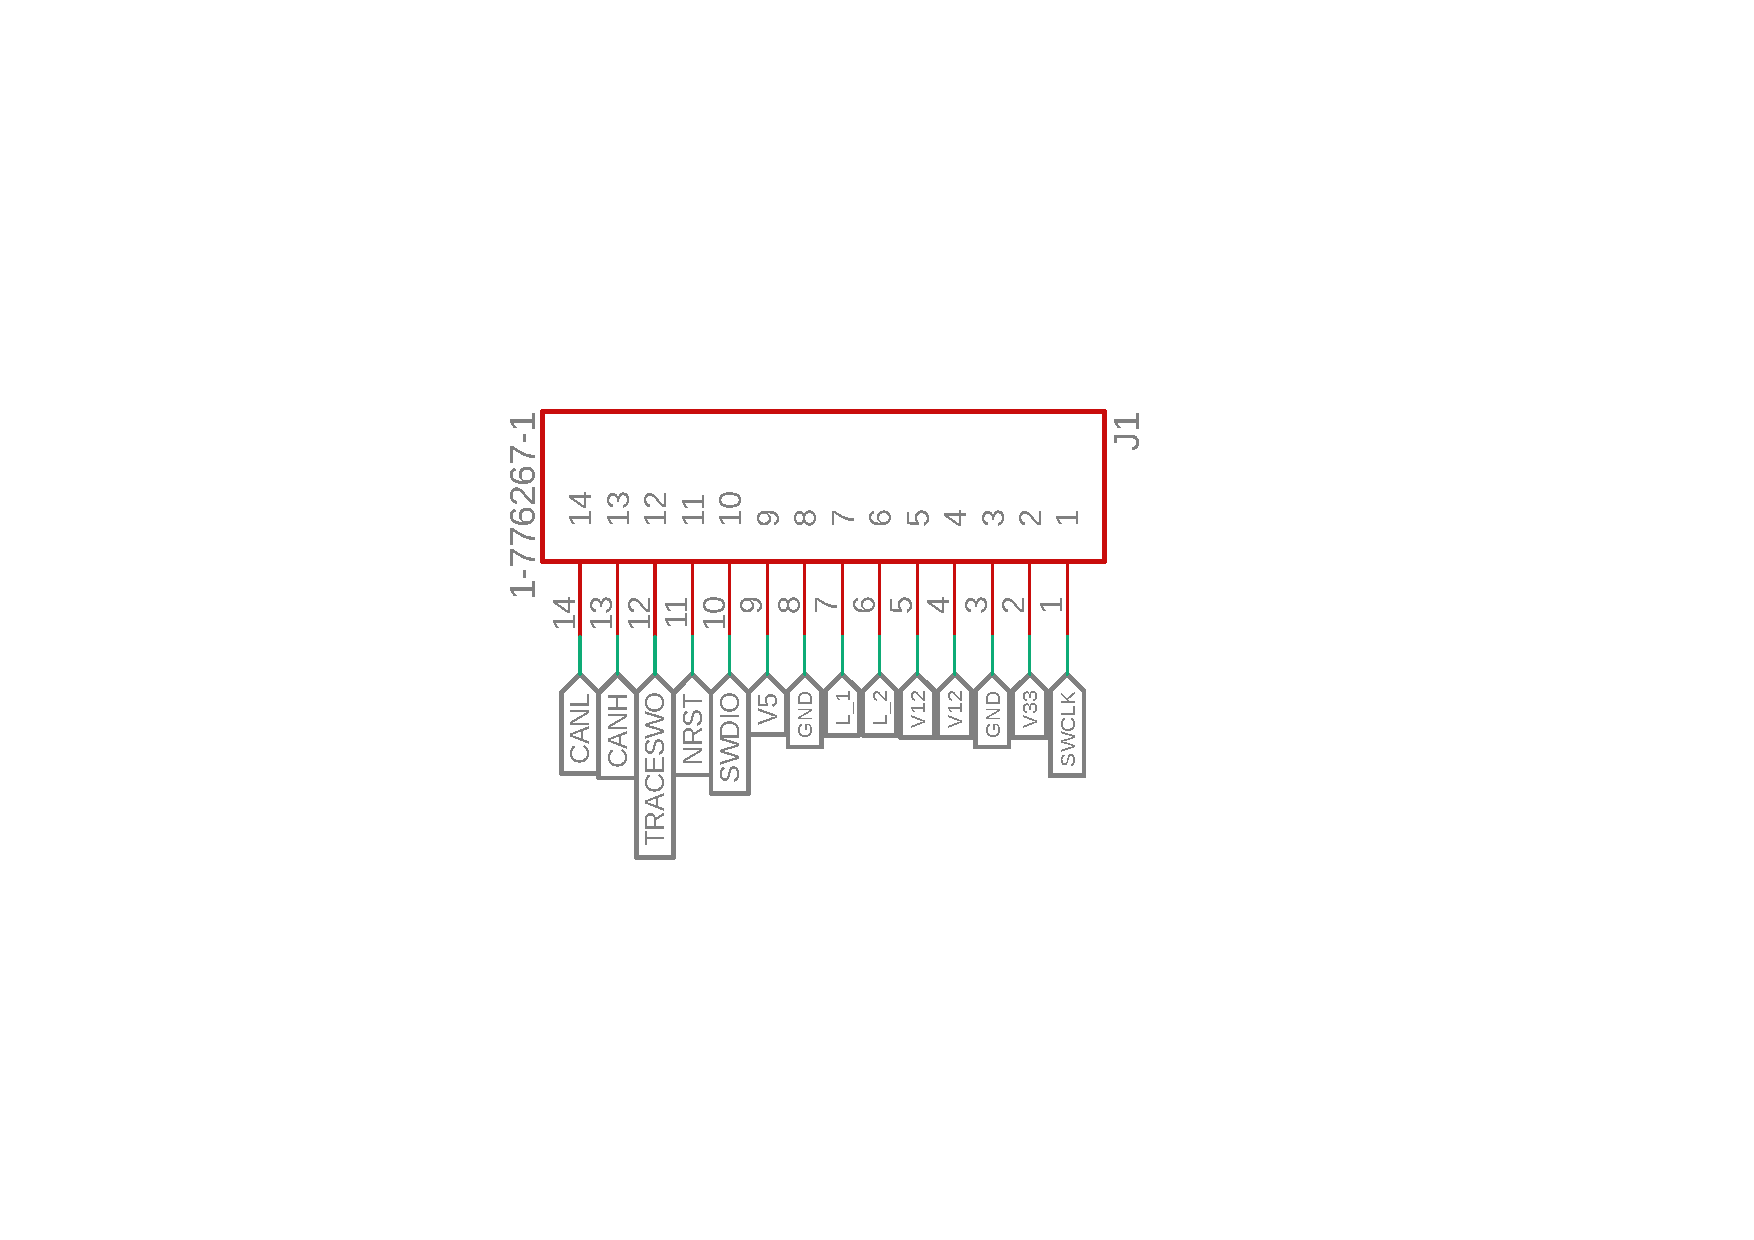
\includegraphics[width=200pt]{./Bilder/stecker.pdf}%
\caption{Anschlusspins Stecker}%
\label{fig:stecker}%
\end{figure}

\section{H-Brücke}\label{sec:hbridge}
Um den Aktor in beide Richtungen  betreiben zu können wird eine elektronische Schaltung benötigt, welche eine Stromrichtungsumkehr ermöglicht. Eine einfache Möglichkeit bietet die sogenannte H-Brückenschaltung, die vereinfacht in \autoref{fig:hbruecke} dargestellt ist. Eine H-Brücke ist eine Vollbrücke bestehend aus vier Schaltern und demnach ein Vierquadrantensteller. Werden die Schalter $S_1$ und $S_4$ geschlossen, kommt es zu einem Stromfluss durch den Aktor. Werden hingegen ausschließlich die Schalter $S_2$ und $S_3$ geschlossen, fließt der Strom entgegengesetzt. Ein Kurzschluss entsteht, wenn $S_1$ und $S_3$ oder $S_2$ und $S_4$ gleichzeitig geschlossen werden. Die Kombination aus Schließung von $S_1$ und $S_2$ oder $S_3$ und $S_4$ resultiert in einem offenen Schaltkreis. \\
\begin{figure} [H]
	\centering
	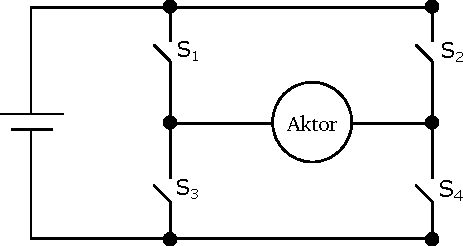
\includegraphics[width=0.3\linewidth]{Bilder/hbruecke.pdf}
	\caption{Vereinfachter Aufbau einer H-Brücke}
	\label{fig:hbruecke}
\end{figure}\noindent
In realen Systemen werden die Schalter durch Transistoren realisiert. Um Kurzschlüsse zu vermeiden, bietet sich die Schaltung einer H-Brücke über zwei Halbbrücken-ICs an. Jede Halbbrücke besteht dabei aus zwei Transistoren, wobei die integrierte Schaltung verhindert, dass beide gleichzeitige durchschalten. Bisher wurde am Aktorprüfstand eine gekaufte H-Brückenschaltung verwenden, die auf zwei \textit{BTS7960}-Halbbrücken der Firma Infineon basiert. Diese lieferte in vorangegangenen Arbeiten zufriedenstellende Leistungsergebnisse. Da sie jedoch  lediglich einen maximalen Stromfluss von \SI{43}{A} zulässt, die Schaltung aber in Zukunft auch für einem Aktor mit \SI{55}{A} benutzt werden soll, kann sie für die zu entwickelnde H-Brücke nicht verwendet werden. Eine Alternative ist die \textit{BTN8982}-Halbbrücke, welche auch von der Firma Infineon produziert wird und für einen maximalen Strom von \SI{55}{A} ausgelegt ist. Das Blockdiagramm dieser Halbbrücken ist in \autoref{fig:btn8982} dargestellt. \\
\begin{figure} [H]
	\centering
	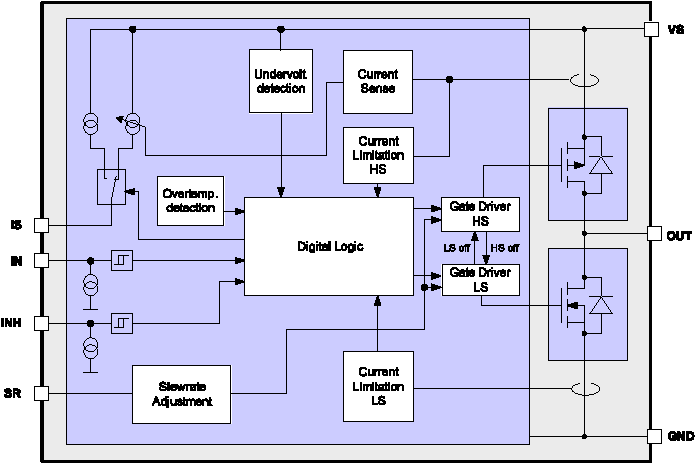
\includegraphics[width=0.65\linewidth]{Bilder/btn8982.pdf}
	\caption{Blockdiagramm der BTN8982 Halbbrücke \cite[S.4]{btn}}
	\label{fig:btn8982}
\end{figure}\noindent
Sie besteht aus einem \textit{p-channel highside MOSFET}, einem \textit{n-channel lowside MOSFET} und einem \textit{Driver IC}, welcher \textit{logic level inputs} unterstützt, wodurch der Anschluss an einen Mikrocontroller erleichtert wird. Die \textit{BTN8982} ist in einem Temperaturbereich von \SI{-40}{^\circ C} bis \SI{150}{^\circ C} einsetzbar und kann mit einer Versorgungsspannung von bis zu \SI{40}{V} betrieben werden, wobei diese im normalen Betrieb zwischen \SI{8}{V} und \SI{18}{V} liegen sollte. Zusätzlich sind mehrere Schutzfunktionen integriert, beispielsweise ein Überstrom- und ein Übertemperaturschutz. Die \textit{BTN8982} besitzt acht Ausgänge, welche in \autoref{tab:Pinverteilung} aufgelistet und im Folgenden näher erläutert werden.

\begin{table}[H]
	\centering
		\captionabove{Pinverteilung Halbbrücken}
		\begin{tabular}{l p{2,5cm} p{8cm} p{3cm}}
			\textbf{Pin Nummer} & \textbf{Bezeichnung} & \textbf{Erläuterung} & \textbf{Anschluss an} \\ \hline
			1 & GND (Ground) & Erdung & Ground MCU \\
			2 & IN (Input) & definiert die Schalterstellung (1 = High Switch Mode; 0 = Low Switch Mode) & O-Pin MCU \\
			3 & INH (Inhibit) & 1: Betriebsmodus, 0: Schlafmodus & O-Pin MCU \\
			4, 8 & OUT (Output) & Ausgang der Brückenschaltung & Aktor \\
			5 & SR (\textit{slew rate}) & Einstellen der Steigung der Spannungsantwort & Ground über Widerstand \\
			6 & IS (Status) & Strommessung \& Fehlererkennung & I-Pin MCU\\
			7 & VS (Supply) & Stromversorgung & Batterie\\
		\end{tabular}
	
	\label{tab:Pinverteilung}
\end{table}\noindent
Pin 1 ist der GND-Pin und bestimmt das Bezugsniveau der Versorgungsspannung, welche an Pin 7 angelegt wird. Ob Strom durch den highside MOSFET oder den lowside MOSFET fließt, wird durch Pin 2 (IN) bestimmt. Liegt eine 1 an fließt Strom durch den highside MOSFET, während bei einer 0 Strom durch letzteren fließt. Wird die Halbbrücke über ein PWM Signal geschaltet, geschieht dies über das Signal an diesem Pin. Der dritte Pin (INH) setzt die Halbbrücke in einen \textit{sleep-mode}, solange eine 0 anliegt. Somit kann die Halbbrücke nur genutzt werden, wenn eine 1 anliegt. Der \textit{sleep-mode} wird als Notaus verwendet, falls die Software einen kritischen Fehler detektiert (siehe \autoref{subsec:MOT}). Pin 4 und 8 (OUT) sind die Pins an die die Versorgungsspannung durchgeschaltet wird und stellen damit die direkte Schnittstelle mit dem Aktor da. Pin 5 (SR) bestimmt die \textit{slew rate} des PWM Signals IN-Pin. Der sechste Pin (IS) ist für die Strommessung, sowie für die Meldung von Fehlern zuständig. Die Funktionsweise ist in \autoref{fig:IS_Pin} dargestellt.\\

\begin{figure} [H]
	\centering
	\includegraphics[width=0.7\linewidth]{Bilder/IS_Pin.pdf}
	\caption{Funktionsweise des IS \cite[S.18]{btn}}
	\label{fig:IS_Pin}
\end{figure}\noindent
Im normalen Operationsmodus (Current Sense Mode) liefert eine integrierte Stromquelle einen Strom $I_{is}$ der proportional zum durchgeschalteten Strom $I_{l}$ ist. Tritt ein Fehler auf, wie zum Beispiel Übertemperatur oder Überstrom, schaltet die Halbbrücke in den Error Flag Mode. Hierbei wird die Stromquelle am IS-Pin gewechselt, welche einen konstanten Strom $I_{IS}$ liefert.  Dieser beträgt maximal \SI{6,5}{mA}. Der Proportionalitätsfaktor $\kappa$ ist durch

\begin{equation}
\kappa = \frac{I_{L1}-I_{L2}}{I_{IS}(I_{L2})-I_{IS}(I_{L1})}
\end{equation}\noindent
definiert und beträgt laut Datenblatt typischerweise 19.500 \cite[S.20]{btn}. Messungen haben gezeigt, dass $\kappa$ in der geschalteten H-Brücke unterhalb dieses Wertes liegt, sodass er als obere Abschätzung des geflossenen Stroms verwendet werden kann.
Die Spannungen an IN- und INH-Pins und somit auch die Funktionalität der H-Brücke wird durch einen Hochgeschwindigkeitsleitungsverstärker/ Puffer (\textit{CD74HCT125}) bereitgestellt. Leitungsverstärker sind elektronische Verstärkerschaltungen, die eingesetzt werden, um die Qualität elektrischer Signale zu verbessern \cite{Conrads2014}. Der schematischer Schaltplan des verwendeten Leitungsverstärkers und die zugehörige Logiktabelle sind in \autoref{fig:buffer} dargestellt. Der \textit{CD74HCT125} besitzt vier unabhängige Wege, die getrennt voneinander aktiviert werden können. Diese Aktivierung geschieht hierbei über ein \textit{Low Level} Spannungssignal am nOE-Pin. Low Level bedeutet, dass die Spannung maximal \SI{1,35}{V} betragen darf. Aufgrund des Platinendesigns (siehe \autoref{kap5}) lässt sich dies recht problemlos bewerkstelligen, was neben der Hitzebeständigkeit und Schnelligkeit das Hauptargument für diesen Leitungsverstärker ist. Ist ein Weg aktiviert, sorgt ein \textit{High Level} Spannungssignal am Eingang (nA) dafür, dass die Versorgungspannung (VCC) an den jeweiligen Ausgang (nY) durchgeschaltet wird. In der ausgeführten Schaltung wird am VCC-Pin des \textit{CD74HCT125} eine Spannung von \SI{5}{V} angelegt. Die ersten drei Wege sind direkt mit GND verbunden, wodurch eine dauerhafte Aktivierung realisiert wird. Die ersten beide Wege sorgen für die Spannung an den IN-Pins der Halbbrücke, während der dritte Weg die INH-Pins versorgt. Die Eingänge sind dabei mit dem Mikrocontroller und die Ausgänge mit den Pins der Halbbrücke verbunden. Somit wird das PWM-Signal des Mikrocontrollers, welches eine maximale Spannung von \SI{3,3}{V} besitzt, auf ein PWM-Signal mit einer maximalen Spannung von \SI{5}{V} angehoben.

\begin{figure}[H]
	\begin{center}
		\noindent\begin{minipage}[h!]{0.45\textwidth} %Beginn der ersten Minipage
			\centering
			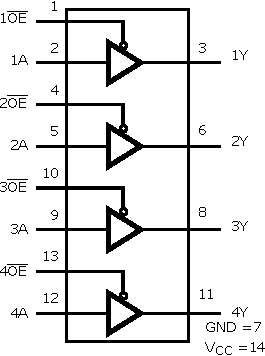
\includegraphics[height=0.85\textwidth]{Bilder/buffer.pdf}
		\end{minipage} %Ende der ersten Minipage
		\quad
		\begin{minipage}[h!]{0.45\textwidth} %Beginn der zweiten Minipage
			\centering
			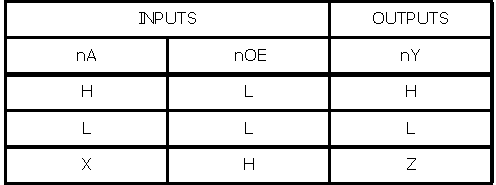
\includegraphics[height=0.3\textwidth]{Bilder/tabelle.pdf}
		\end{minipage} %Ende der zweiten Minipage
	\end{center}
	\caption{Schematischer Aufbau und Logiktabelle des CD74HCT125 Leitungsverstärkers \cite[S.2]{Buffer}}
	\label{fig:buffer}
\end{figure}\noindent
Die H-Brücke kann auch ohne einen Leitungsverstärker direkt mit dem Mikrocontroller verbunden werden, was zur Folge hätte, dass keine \SI{5}{V} sondern \SI{3,3}{V} Spannung an den Pins der H-Brücke anliegen. \autoref{fig:Strommessung} zeigt den geflossenen Strom durch den dabei angeschlossenen Aktor mit und ohne Leitungsverstärker bei variierenden PWM-Signalen. Es ist zu sehen, dass die Messung mit geschaltetem Leitungsverstärker deutlich symmetrischer sind, was auf eine bessere bidirektionale Schaltbarkeit schließen lässt. Außerdem sind die maximal durchgeschalteten Ströme größer. Dies lässt vermuten, dass die \SI{3,3}{V} nicht ausreichen, um die Transistoren in den Halbbrücken vollständig schalten zu lassen. Dementsprechend wurde sich bei der endgültigen Schaltung für den Einsatz eines Leitungsverstärkers entschieden. 

\begin{figure} [H]
	\centering
	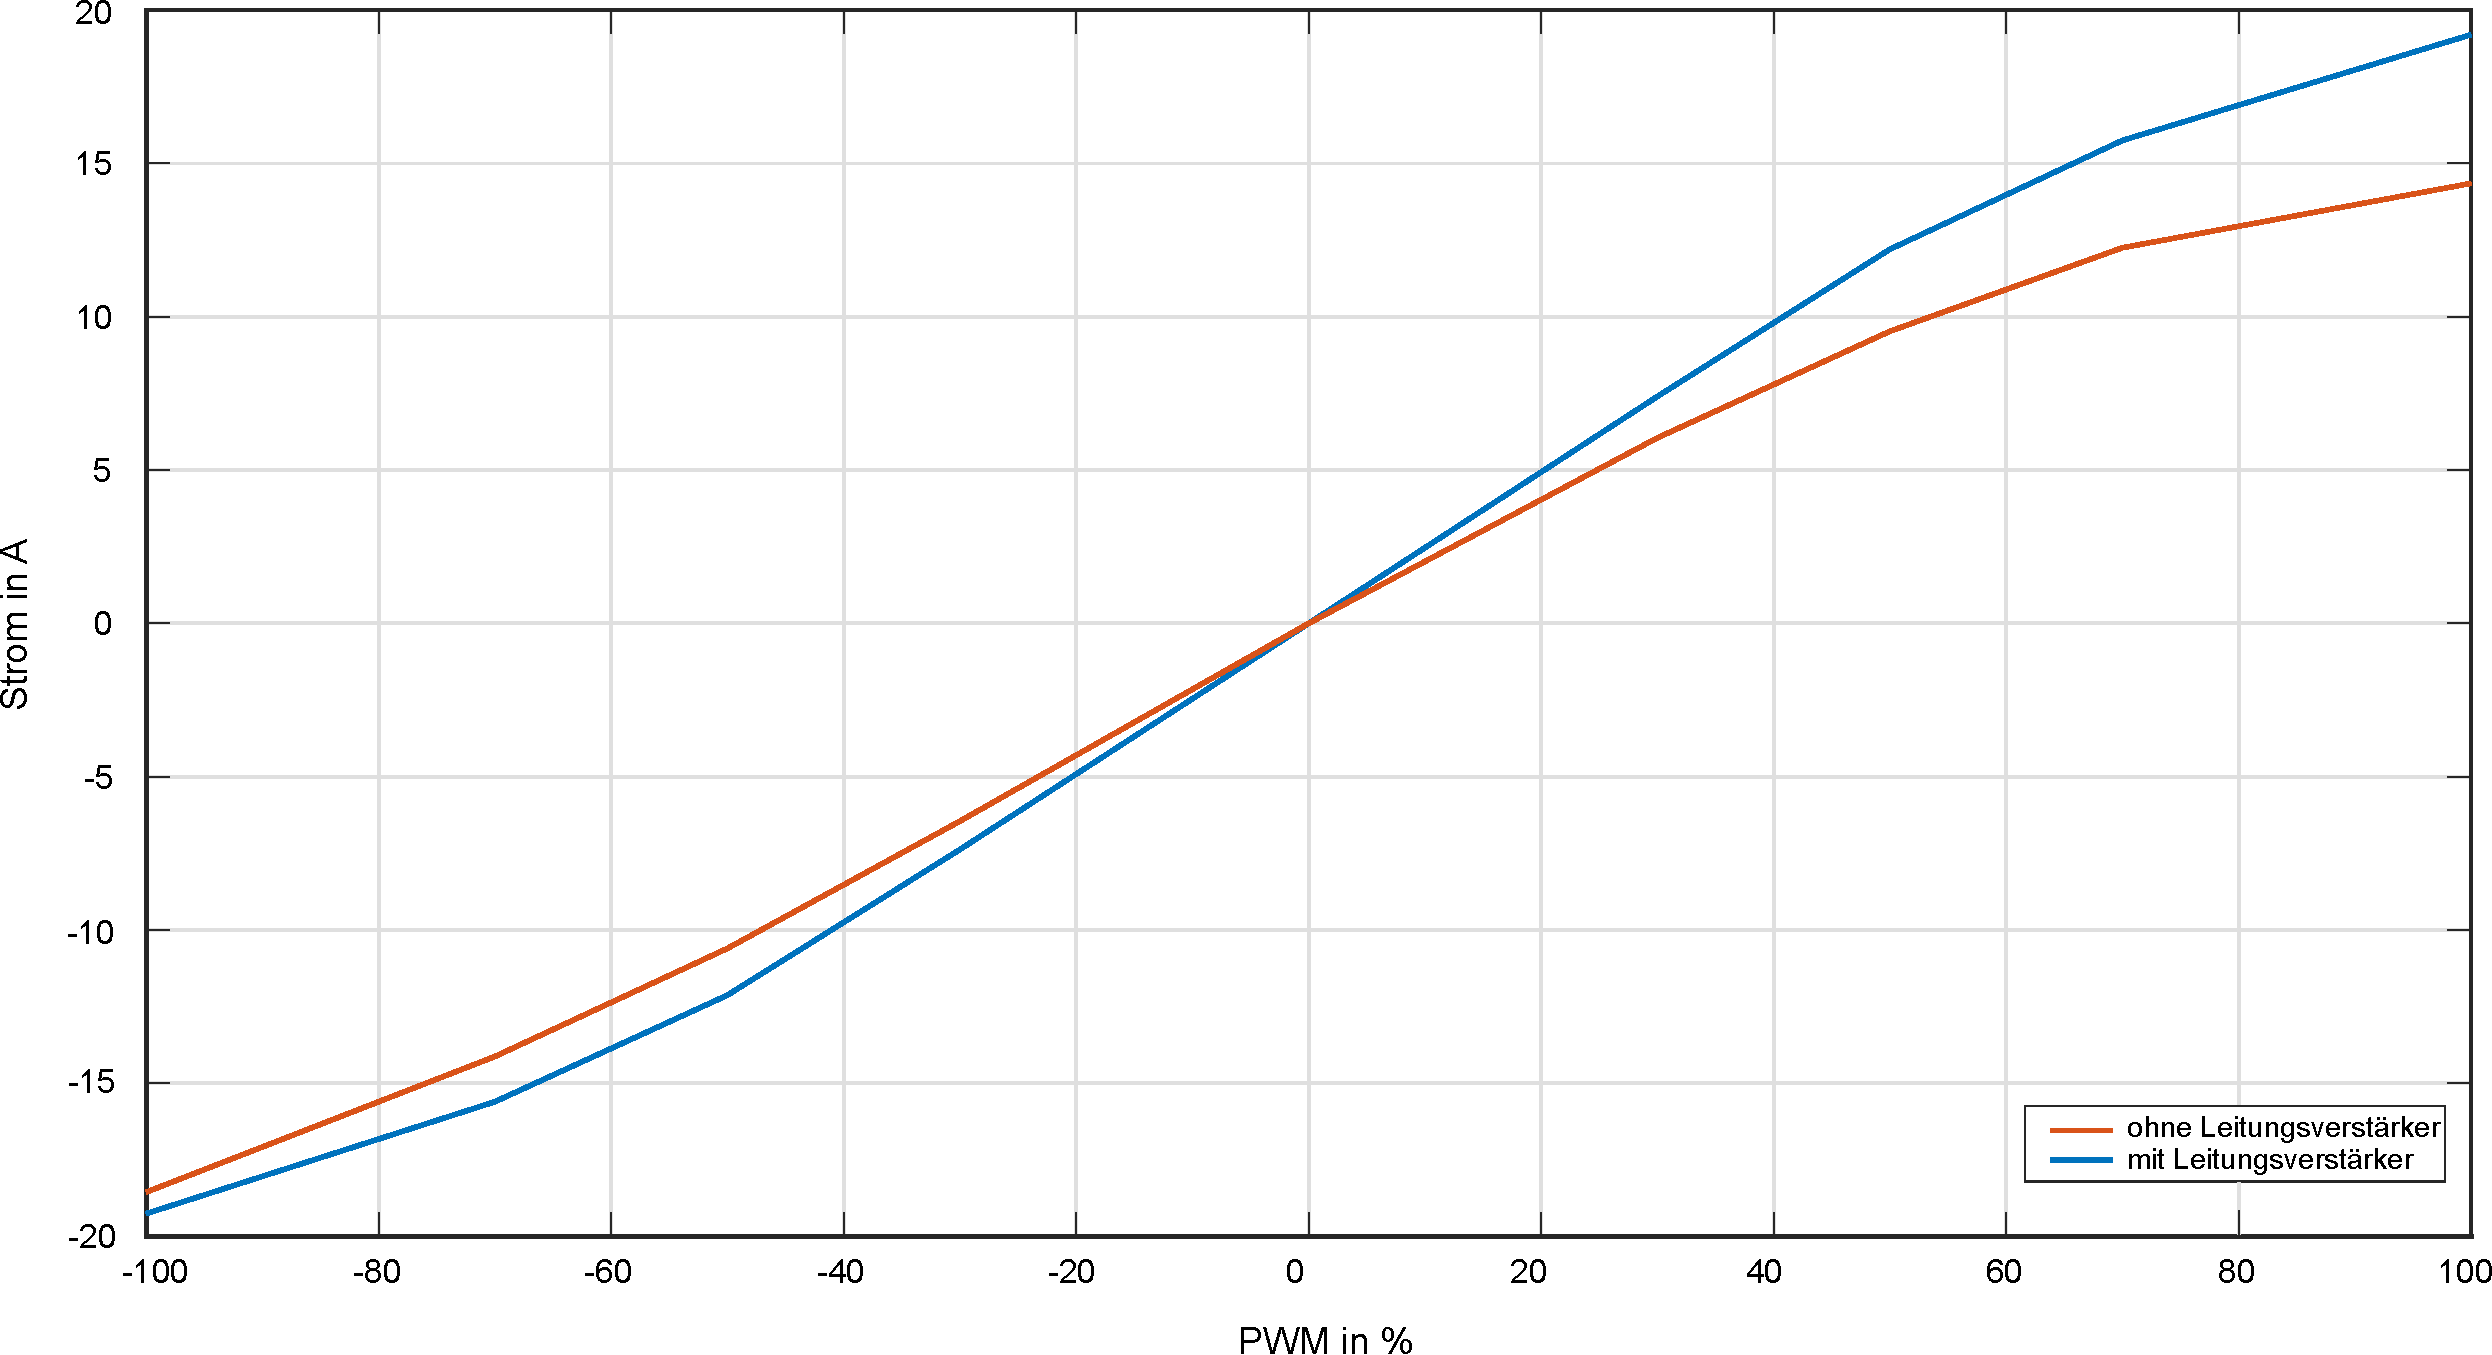
\includegraphics[width=0.8\linewidth]{Bilder/Strommessung.pdf}
	\caption{Strommessung mit und ohne Leitungsverstärker bei unterschiedlichen PWM-Signalen}
	\label{fig:Strommessung}
\end{figure}\noindent
Der schematische Aufbau der verwendeten H-Brücke ist in \autoref{fig:schematisch_hbruecke} zu sehen und wird im Folgenden genauer erläutert. Bei dem hier vorgestellten Aufbau wurde sich am Datenblatt der \textit{BTN8982}-Halbbrücken orientiert \cite[S.22]{btn}.

\begin{figure} [H]
	\centering
	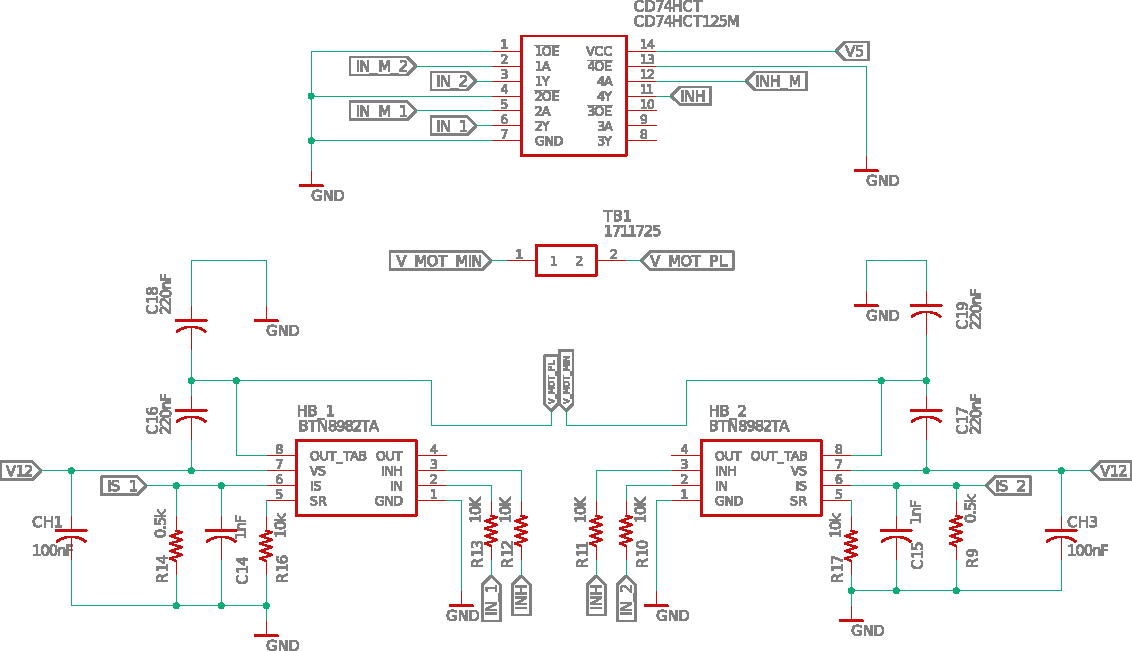
\includegraphics[width=1\linewidth]{Bilder/schematisch_hbruecke.pdf}
	\caption{Schematischer Aufbau der H-Brücke}
	\label{fig:schematisch_hbruecke}
\end{figure}\noindent
An beiden Halbbrücken wird am VS-Pin die Versorgungsspannung angelegt. Nahe am jeweiligen VS-Pin ist ein \SI{100}{nF} Kondensator (CH1, CH3) gegen GND geschaltet, welcher die Schwankungen der Versorgungsspannung, z.B. verursacht durch andere Komponenten, glättet. Ob diese Spannung an die OUT-Pins durchgeschaltet wird, hängt von der Spannung an den IN- und INH-Pins ab. Die INH-Pins setzen die Halbbrücken in einen \textit{sleep-mode}, wenn an ihnen keine Spannung zwischen 3 und \SI{5,3}{V} angelegt ist. Sofern diese Spannung anliegt, sorgt der gleiche Spannungsbereich am IN-Pin dafür, dass die Versorgungsspannung an die OUT-Pins der Halbbrücke durchgeschaltet wird. Jede Halbbrücke besitzt zwei solcher OUT-Ausgänge, wobei einer über einen Pin und der andere über eine große Fläche auf der Rückseite realisiert wird. Letzterer eignet sich besser zum Übertragen großer Ströme, weshalb dieser zur Aktoransteuerung verwendet wird.  Die IN- und INH-Pins werden über \SI{10}{k\Omega} Widerstände (R10, R11, R12, R13) mit den Ausgängen des Leitungsverstärkers verbunden. Diese Widerstände werden zum Schutz der digitalen Eingänge benötigt.
Die IS-Pins der Halbbrücke werden direkt mit dem Mikrocontroller verbunden. Parallel sind \SI{0,5}{k\Omega} (R9, R14), sowie ein  \SI{1}{nF} Glättungskondensator (C14, C15) gegen GND geschaltet. Diese Pins sind für die Sensorik der Halbbrücke verantwortlich. An ihnen ist eine Stromquelle angeschlossen, die einen zum durchgeschalteten Strom proportionalen Strom liefert. Abhänging von den gegen GND geschalteten Widerständen ergibt sich eine Spannung die vom Mikrocontroller gemessen und aus der der durchgeschaltete Strom berechnet werden kann. Da der Strom am IS-Pin maximal \SI{6,5}{mA} beträgt, resultiert durch einen \SI{0,5}{k\Omega} eine maximale Spannung von \SI{3,25}{V} am Mikrocontroller. Ein größerer Widerstand hätte eine größere Spannung zur Folge, wodurch eine Schädigung des Mikrocontrollers nicht mehr ausgeschlossen werden kann. 
Die Widerstände, die zwischen SR-Pins und GND geschaltet sind (R16, R17), bestimmen die \textit{slew rate} des durchgeschalteten Signals. Dieser darf laut Datenblatt zwischen \SI{0}{\Omega} und \SI{51}{k\Omega} liegen. Der Hersteller bietet zudem eine Simulation an, in der verschiedene \textit{slew rate}-Widerstände getestet werden können. Die Ergebnisse einer solchen Simulation mit den eingestellten Widerständen \SI{0}{\Omega}, \SI{10}{k\Omega} und \SI{51}{k\Omega} sind anhand des durchgeschalteten Stroms $I_{OUT}$ in \autoref{fig:Simulationsergebnisse} dargestellt. Es ist zu sehen, dass der durchgeschaltete Strom mit zunehmendem Widerstand abnimmt, die Welligkeit jedoch nahezu gleich bleibt. Allerdings gilt es zu beachten, dass die \textit{Electromagnetical Interference} (kurz: EMI) für kleinere \textit{slew rate}-Widerstände ansteigt. Ein Widerstand von \SI{10}{k\Omega} stellt dabei einen guten Kompromiss dar und liefert auch in realen Messungen sehr gute Ergebnisse.
\begin{figure} [H]
	\centering
	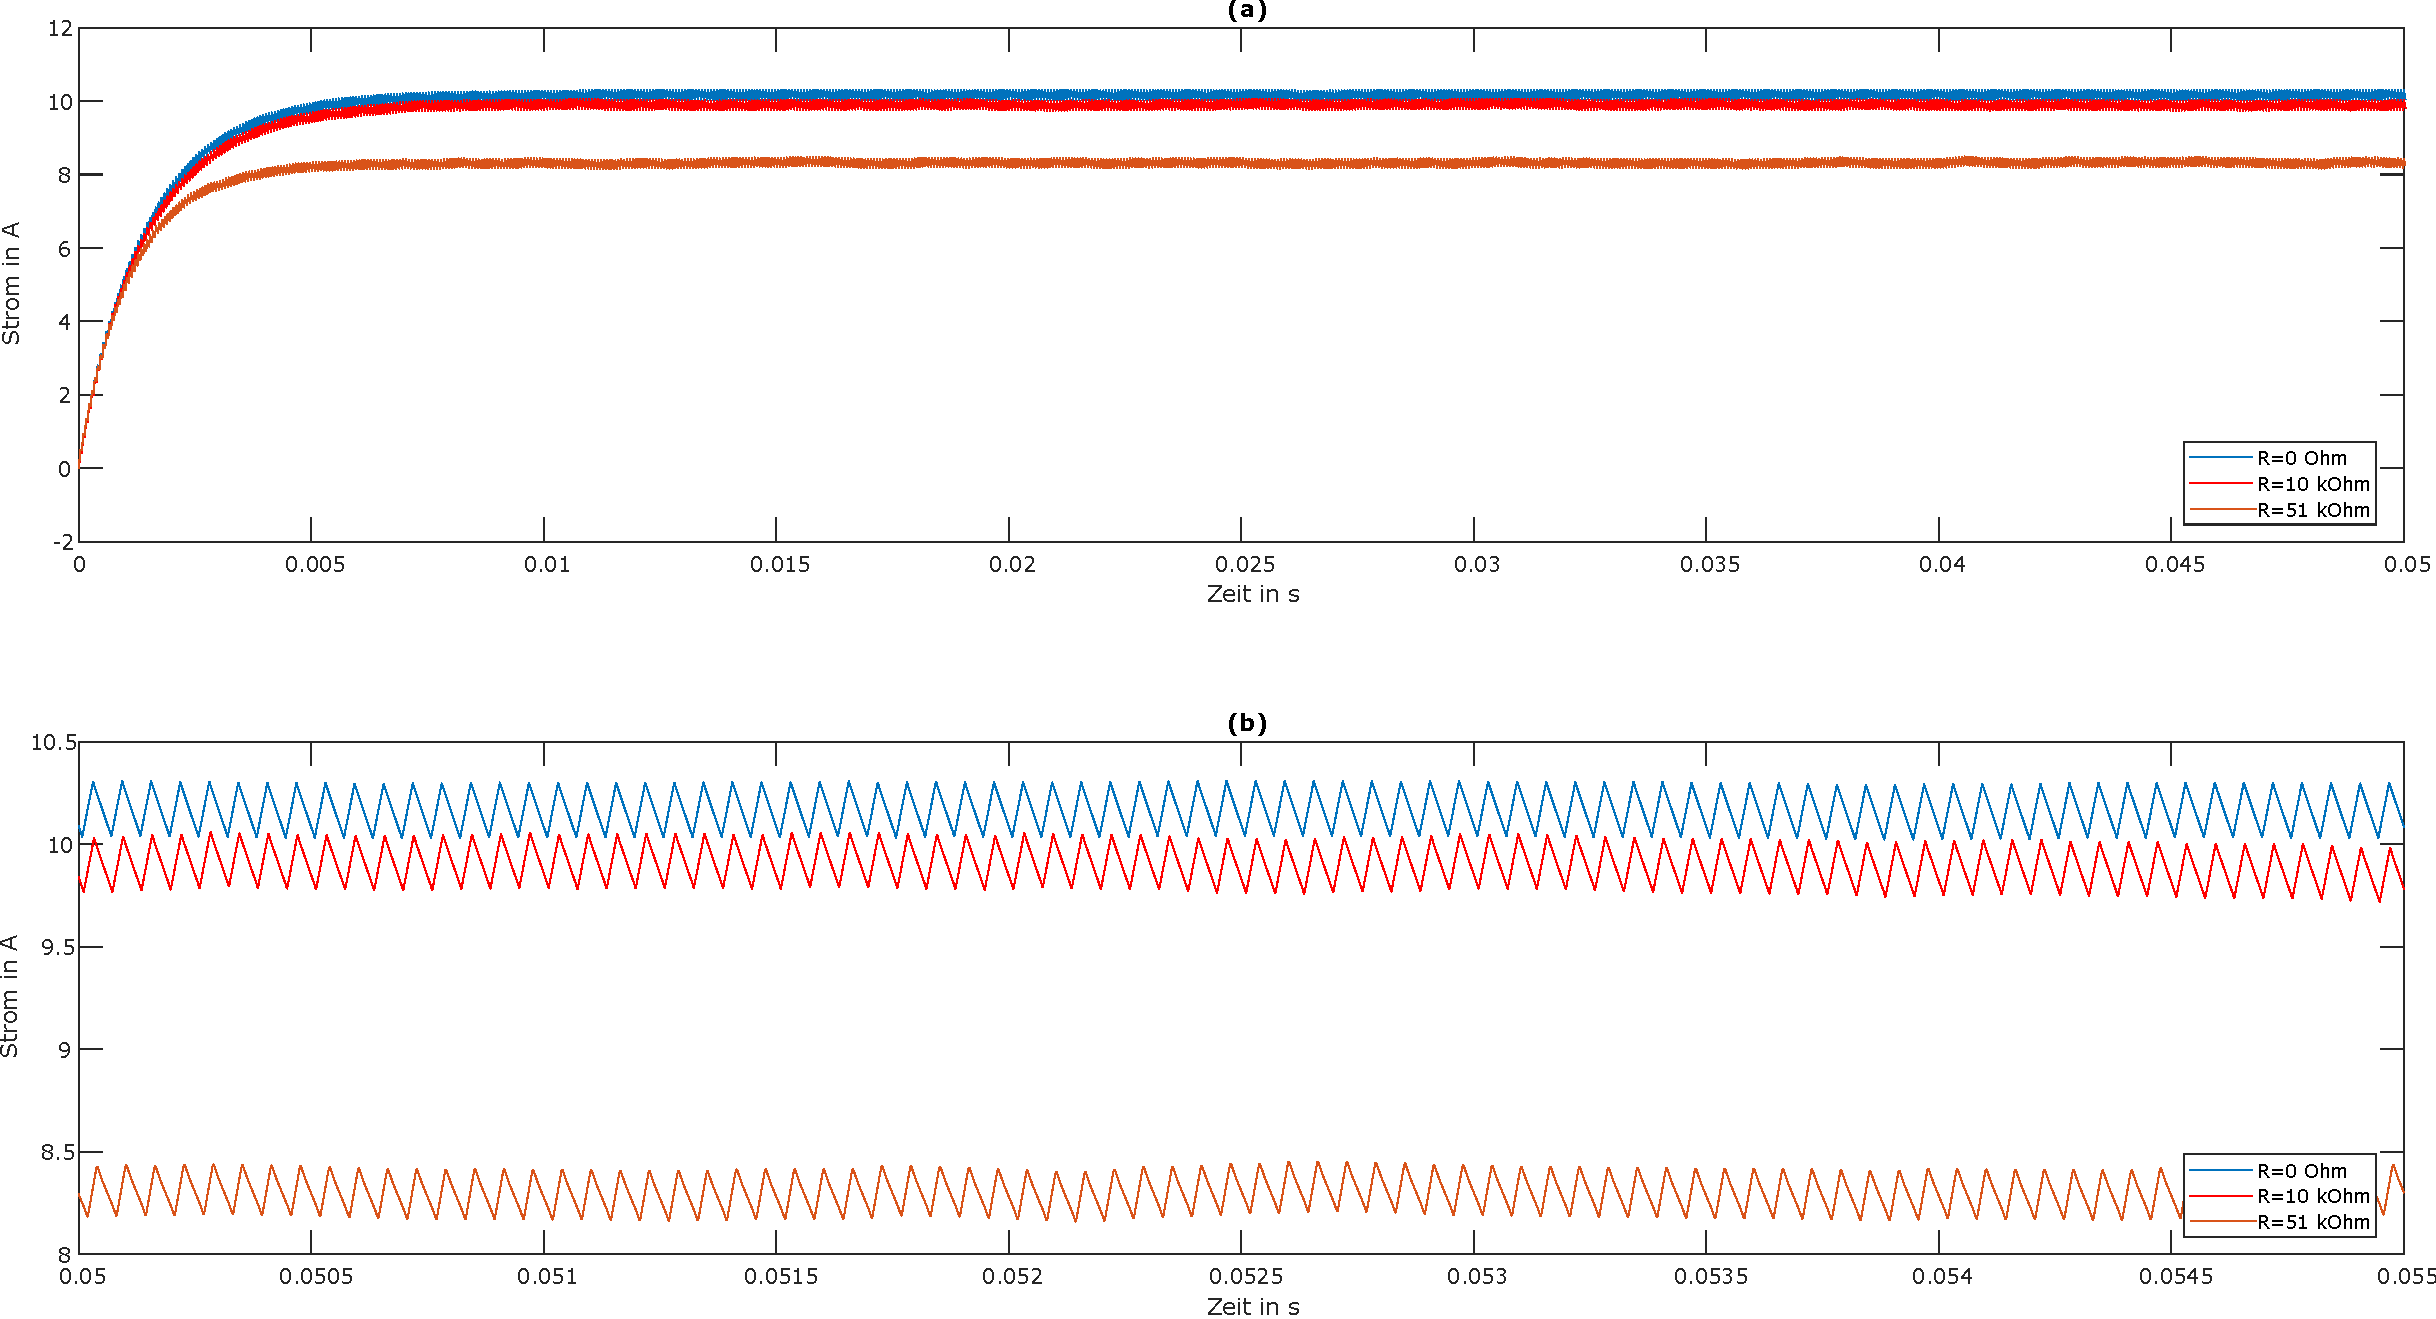
\includegraphics[width=1\linewidth]{Bilder/Simulationsergebnisse.pdf}
	\caption{(a):Simulationsergebnisse des durchgeschalteten Stroms über der Zeit aufgetragen; (b): Welligkeit des durchgeschalteten Stroms}
	\label{fig:Simulationsergebnisse}
\end{figure}\noindent
Bei der Simulation, sowie auch in der realen Anwendung, beträgt die Schaltfrequenz \SI{16}{kHz}. Dabei wurde sich an der vorangegangenen Arbeit orientiert, wobei auch höhere (\SI{20}{kHz}) und niedrige Frequenzen (\SI{10}{kHz}) getestet wurden. Höhere Schaltfrequenzen bieten prinzipiell den Vorteil, dass die Welligkeit des durchgeschalteten Stroms abnimmt. Allerdings steigt dabei auch die EMI. Der Unterschied der Welligkeit zwischen \SI{16}{kHz} und \SI{20}{kHz} ist jedoch vernachlässigbar klein, weshalb sich für die geringe EMI entschieden wurde. Im Gegensatz dazu ist bei \SI{10}{kHz} die Zunahme der Welligkeit deutlich zu beobachten.  

\section{Sensorik}
Die Sensorik des Gesamtsystems besteht aus einem Stromsensor, einem Temperatursensor und einem Lagesensor. Während die ersten beiden wichtige Kontroll- und Leistungsgrößen liefern, ist der Lagesensor essentiell für die Schaltvorgänge und damit die Funktionalität des Gesamtsystems. Der Stromsensor ist in den BTN8982 Halbbrücken integriert und ist bereits beschrieben. Die Funktionsweise und Verschaltung des Temperatur- und Lagesensors werden im folgenden erläutert. 

\subsection{Temperatursensor}\label{sub:temp}
Als Temperatursensor wird ein \textit{B57861S0103A039}-Thermistor verwendet. Dieser besteht aus einem Sensor und zwei \SI{350}{mm} langen Anschlusskabeln. Thermistoren sind elektrische Widerstände, deren Wert temperaturabhängig variiert. Dabei werden sie in die zwei Gruppen Heiß- und Kaltleiter aufgeteilt \cite{Stiny2015}. Da der \textit{B57861S0103A039}-Thermistor zur ersten Gruppe gehört, wird im folgenden ausschließlich auf diese eingegangen. Heißleiter besitzen einen negativen Temperaturkoeffizient (NTC), was bedeutet, dass ihr elektrische Widerstand sich mit steigender Temperatur reduziert. Dieser Zusammenhang ist allerdings hochgradig nichtlinear und kann durch 

\begin{equation} \label{eq:NTC}
R(T) = R_R \cdot e^{\beta\left(\frac{1}{T}-\frac{1}{T_R}\right)}  
\end{equation}
beschrieben werden mit der Referenztemperatur $T_R$, dem Widerstand $R_R$ bei der Referenztemperatur und dem Beta-Wert $\beta$. Als Referenztemperatur wird meistens \SI{25}{^\circ C} gewählt. Der Beta-Wert ist eine Materialkonstante, die üblicherweise zwischen \SI{1500}{K} und \SI{6000}{K} liegt \cite{Stiny2015}. Für den \textit{B57861S0103A039}-Thermistor beträgt der Widerstand $R_R$ \SI{10}{k\Omega} und der Beta-Wert $\beta$ \SI{3988}{K}. Der Betriebstemperatur liegt zwischen \SI{-55}{^\circ C} und \SI{155}{^\circ C}, was in den typischen Bereich für Heißleiter fällt \cite{Stiny2015}.\\
Eine mögliche Schaltung zur hochgenauen Temperaturmessung mittels Heißleitern ist die Wheatstonsche-Brückenschaltung (\autoref{fig:wheatstone}) bestehend aus drei ohmschen Widerständen und einem NTC-Thermistor \cite{Stiny2015}.

\begin{figure} [h]
	\centering
	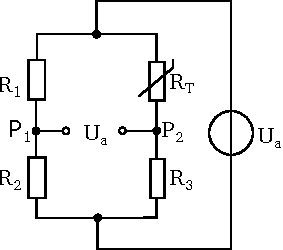
\includegraphics[width=0.4\linewidth]{Bilder/wheatstone.pdf}
	\caption{Wheatstone-Brückenschaltung nach \cite[S.12]{Weissgerber2018}}
	\label{fig:wheatstone}
\end{figure}\noindent
Solange die Brücke ausgeglichen ist, liegt keine Spannungsdifferenz zwischen $P_1$ und $P_4$ vor. Ändert sich der Widerstand des Thermistors, wird der ausgeglichene Zustand verlassen und es kommt zu einer Spannungsdifferenz, aus der der veränderte Widerstand des Thermistors bestimmt werden kann. Wird \autoref{eq:NTC} nach der Temperatur $T$ umgestellt, lässt sich daraus die aktuelle Temperatur berechnen. Aus Platzgründen auf der endgültigen Platine und da die hiermit erzielbare Genauigkeit nicht benötigt wird, ist stattdessen ein Spannungsteiler zum Einsatz gekommen. Dieser Spannungsteiler teilt die am Thermistor und an einem festen Widerstand abfallende Spannung und ist in \autoref{fig_ther_elek} dargestellt. Aus der Spannung, die am konstanten Widerstand $R_c$ abfällt, kann auf die Spannung geschlossen werden, die am Thermistor $R_t$ abfällt und somit auch auf dessen aktuellen Widerstand. Über \autoref{eq:NTC} ist dann ein direkter Zusammenhang zur gemessenen Temperatur gegeben.
Die Spannungsmessung findet im Mikrocontroller bzw. in dessen Analog-Digital-Convertern (ADC) statt. Dabei sind für eine möglichst exakte Messung mehrere Umstände zu beachten, die nun exemplarisch erörtert werden. Die Überlegungen gelten jedoch auch für die übrigen Spannungsteiler und ADCs. Im STM32F4 kommen \textit{successive approximation analog-to-digital converter} zum Einsatz, die eine Auflösung von bis zu \SI{12}{bit} liefern \cite{stmref}. Die Messdauer ist dabei konfigurierbar, entspricht jedoch mindestens für jedes Auflösungs-Bit und 3 zusätzliche Takte (12 + 3 Takte)\cite[S.397]{stmref}. Dieser Takt $f_{ADC}$ entspricht dabei nicht dem Kerntakt, sondern dem \textit{Advanced Peripheral Bus Clock} (APBC), der sich durch konfigurierbare Takt-Teiler vom Kerntakt unterscheidet. \\
Durch den Aufbau des ADC's bedingt, führen zu große Eingangswiderstände (bzw. Widerstandswerte im Spannungsteiler) zu großen Ungenauigkeiten. Dies ist umso kritischer je kürzer die Messdauer beträgt, da sich die interne Kapazität im ADC bei großen Eingangswiderständen nur langsam aufladen kann. Nach Ablauf der Abtastdauer sollte  jedoch die interne Kapazität auf die tatsächlichen Spannung am Eingangspin aufgeladen sein, sonst kommt es zu Abweichungen (siehe dazu auch \cite{ADC}, \cite{stm32}). ST stellt für den Mikrocontroller \autoref{eq:ADC} bereit, durch welche sich der maximale Eingangswiderstand 
\begin{equation} \label{eq:ADC}
R_{AIN} = \frac{(k-0,5)}{f_{ADC} C_{ADC} ln(2^{N+2})} - R_{ADC}
\end{equation}
abhängig der Messdauer berechnen lässt. Dabei entspricht $k$ den konfigurierten Messtakten pro Messung, $C_{ADC}$ der Kapazität des internen ADCs, $N$ der Auflösung und $R_{ADC}$ dem Schaltwiderstand des ADCs. Über $k$ und $f_{ADC}$ lässt sich dabei die Messdauer beeinflussen und somit die erlaubten Eingangswiderstände am Spannungsteiler beeinflussen. Für eine effektive Messdauer von \SI{2,7}{\mu s} muss der Eingangswiderstand unter \SI{31,355}{k\Omega} liegen, während bei einer Messdauer von nur \SI{1,5}{\mu s} nur Eingangswiderstände bis \SI{440,6}{\Omega} für hohe Genauigkeit zulässig sind. Der Nachteil niedrigerer Widerstände im Spannungsteiler liegt jedoch in der Belastung des jeweiligen Sensorausgangs. Dort kann nur ein begrenzter Strom bereit gestellt werden. Daher bietet es sich an, eine Kapazität parallel zum Eingang des ADCs und somit zu $C_{ADC}$ zu schalten, die als Puffer für $C_{ADC}$ dient \cite{ADC}. Hier muss jedoch beachtet werden, dass eine weitere Kapazität zusätzlichen Bauraum, Kosten und Fehlerpotential zur Folge hat. Darüber hinaus werden schnelle Signaländerungen durch die RC-Zeitkonstante zum Auf-/Entladen des Kondensators ggf. herausgefiltert. Für den Thermistor werden keine kritischen Temperatursprünge erwartet, daher wird in diesem Fall eine zusätzliche Kapazität $C_c$ eingesetzt.\\
Auch durch einen Impedanzwandler, also eine Operationsverstärkerschaltung mit einer Spannungsverstärkung von $1$, lässt sich der Eingangswiderstand durch den Spannungsteiler kompensieren. Auch hier ergeben sich jedoch Nachteile durch benötigten Bauraum, anfallende Kosten, gesteigertes Fehlerpotential und zusätzliches Rauschen.\\
\begin{figure}[H]
	\centering
	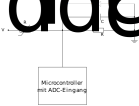
\includegraphics[width=0.5\linewidth]{./Bilder/fig_ther_elek}
	\caption{Schaltung zum Auslesen des Thermistors}
	\label{fig_ther_elek}
\end{figure}\noindent
Durch den Temperatursensor soll die Spulentemperatur im Tauchspulenaktor gemessen werden, da hier durch eine Überhitzung der Isolation Gefahrenpotential ausgeht. In der Umgebung der Spulen wird jedoch eine große Induktionswirkung erwartet, die die Genauigkeit der Spannungsmessung gefährden oder sogar ganz außerhalb des Messbereichs von \SI{0}{V} bis \SI{3,3}{V} liegen und somit die Funktionsfähigkeit des Mikrocontrollers gefährden \cite{stm32}. Eine Gegenmaßnahme stellt die Verseilung der Zuleiterkabel dar. Darüber hinaus kann durch die Schirmung der Kabel eine Schirmdämpfung erreicht werden, was die Induktionswirkung weiter reduziert \cite{Wolfsperger}. Falls trotzdem eine Spannung induziert wird, kann ein  Strom im mA-Bereich über interne Dioden im ADC abgeleitet werden \cite{stmref}. Um den Strom zu begrenzen, muss sich ein Widerstand zwischen induzierter Spannung und ADC-Eingang befinden. Eine weitere Methode den Pin vor einer Überspannung zu schützen, stellt eine Zener-Diode dar, die parallel zum Eingang des ADC's geschaltet wird (grau angedeutet). Hierbei ist jedoch darauf zu achten, dass auch im Normalbetrieb ein Kriechstrom durch die Diode fließt, der das Messergebnis verfälschen kann. \\
Um Probleme dieser Art zu umgehen, wurden auch alternative Sensorkonzepte in Betracht gezogen, die nicht über ein ADC ausgewertet werden. Diese haben sich jedoch als zu rechenaufwändig beim Auslesen erwiesen.

\subsection{Lagesensor}
Die Funktionsweise des PLCS-25M Sensors ist in \autoref{kap2} bereits erläutert worden. Der Sensor gibt demnach ein Spannungssignal aus, das nach \autoref{eq:Lage} in den Schaltgabelweg umgerechnet werden kann. Hierbei ist zu beachten, dass der Lagesensor mit \SI{5}{V} Gleichspannung betrieben wird und demnach der mögliche Ausgangsspannungsbereich zwischen \SI{0}{V} und \SI{5}{V} liegt, was außerhalb des gültigen Messbereichs der ADCs liegt. Über einen Spannungsteiler wird die Ausgangsspannung des Lagesensors demnach in den gültigen Messbereich übersetzt. Es gelten dabei bei der Auslegung des Spannungsteilers die gleichen Überlegungen wie in \autoref{sub:temp}. Um darüber hinaus eine Verbesserung der Positionsbestimmung zu erreichen, wird auch der komplementäre Ausgang des Lagesensors gemessen und entsprechend verrechnet. Der dadurch erreichte Genauigkeitsgewinn wird in \autoref{kap7} thematisiert.

\subsection{Sensorik Eingangsspannung}\label{eingangsspannung}
Um Fehlerzustände in der Spannungsversorgung feststellen zu können, ist ein einfacher Spannungsteiler zu entwerfen, anhand dessen die Eingangsspannung in einen für den ADC lesbaren Bereich gebracht wird. Es gelten die gleichen Überlegungen wie in \autoref{sub:temp}.

